\subsection{Front-End}
For the front-end, we chose a web application, written in Python. 
We did not offer the choice for a different approach in the questionnaire, as a web application offers the most flexibility. 
The admin is able to configure the desired information, and the actual users of the front-end do not need to concern about it.
Another advantage is that no additional software has to be installed on the computers in the medical institution. 
Front-end users only need to open an arbitrary internet browser and navigate to the front-end page. 
Furthermore, in case the front-end needs to be updated, one has not to update the software on each computer. 

\subsubsection{Design}
We offered various design options for the front-end in the questionnaire. 
In the end, the most popular design is illustrated in \ref{fig:gray-color}. 
Potential decubitus patients are marked in red, showing the user that he requires additional attention.
If the user clicks on a red marked patient, a text appears, describing why DecubiTection decided that the patient may develop a decubitus. 
On the other hand, if the user clicks on a gray marked patient, a text appears that no risks concerning decubitus are found, but that there may be still a residual risk, as the detection algorithm is not perfectly accurate. 
In case, the user is confused by the front-end, we included a help button, illustrated in \ref{fig:help}, which describes how to use the software. 

\begin{figure}[htp]
    \centering
    \frame{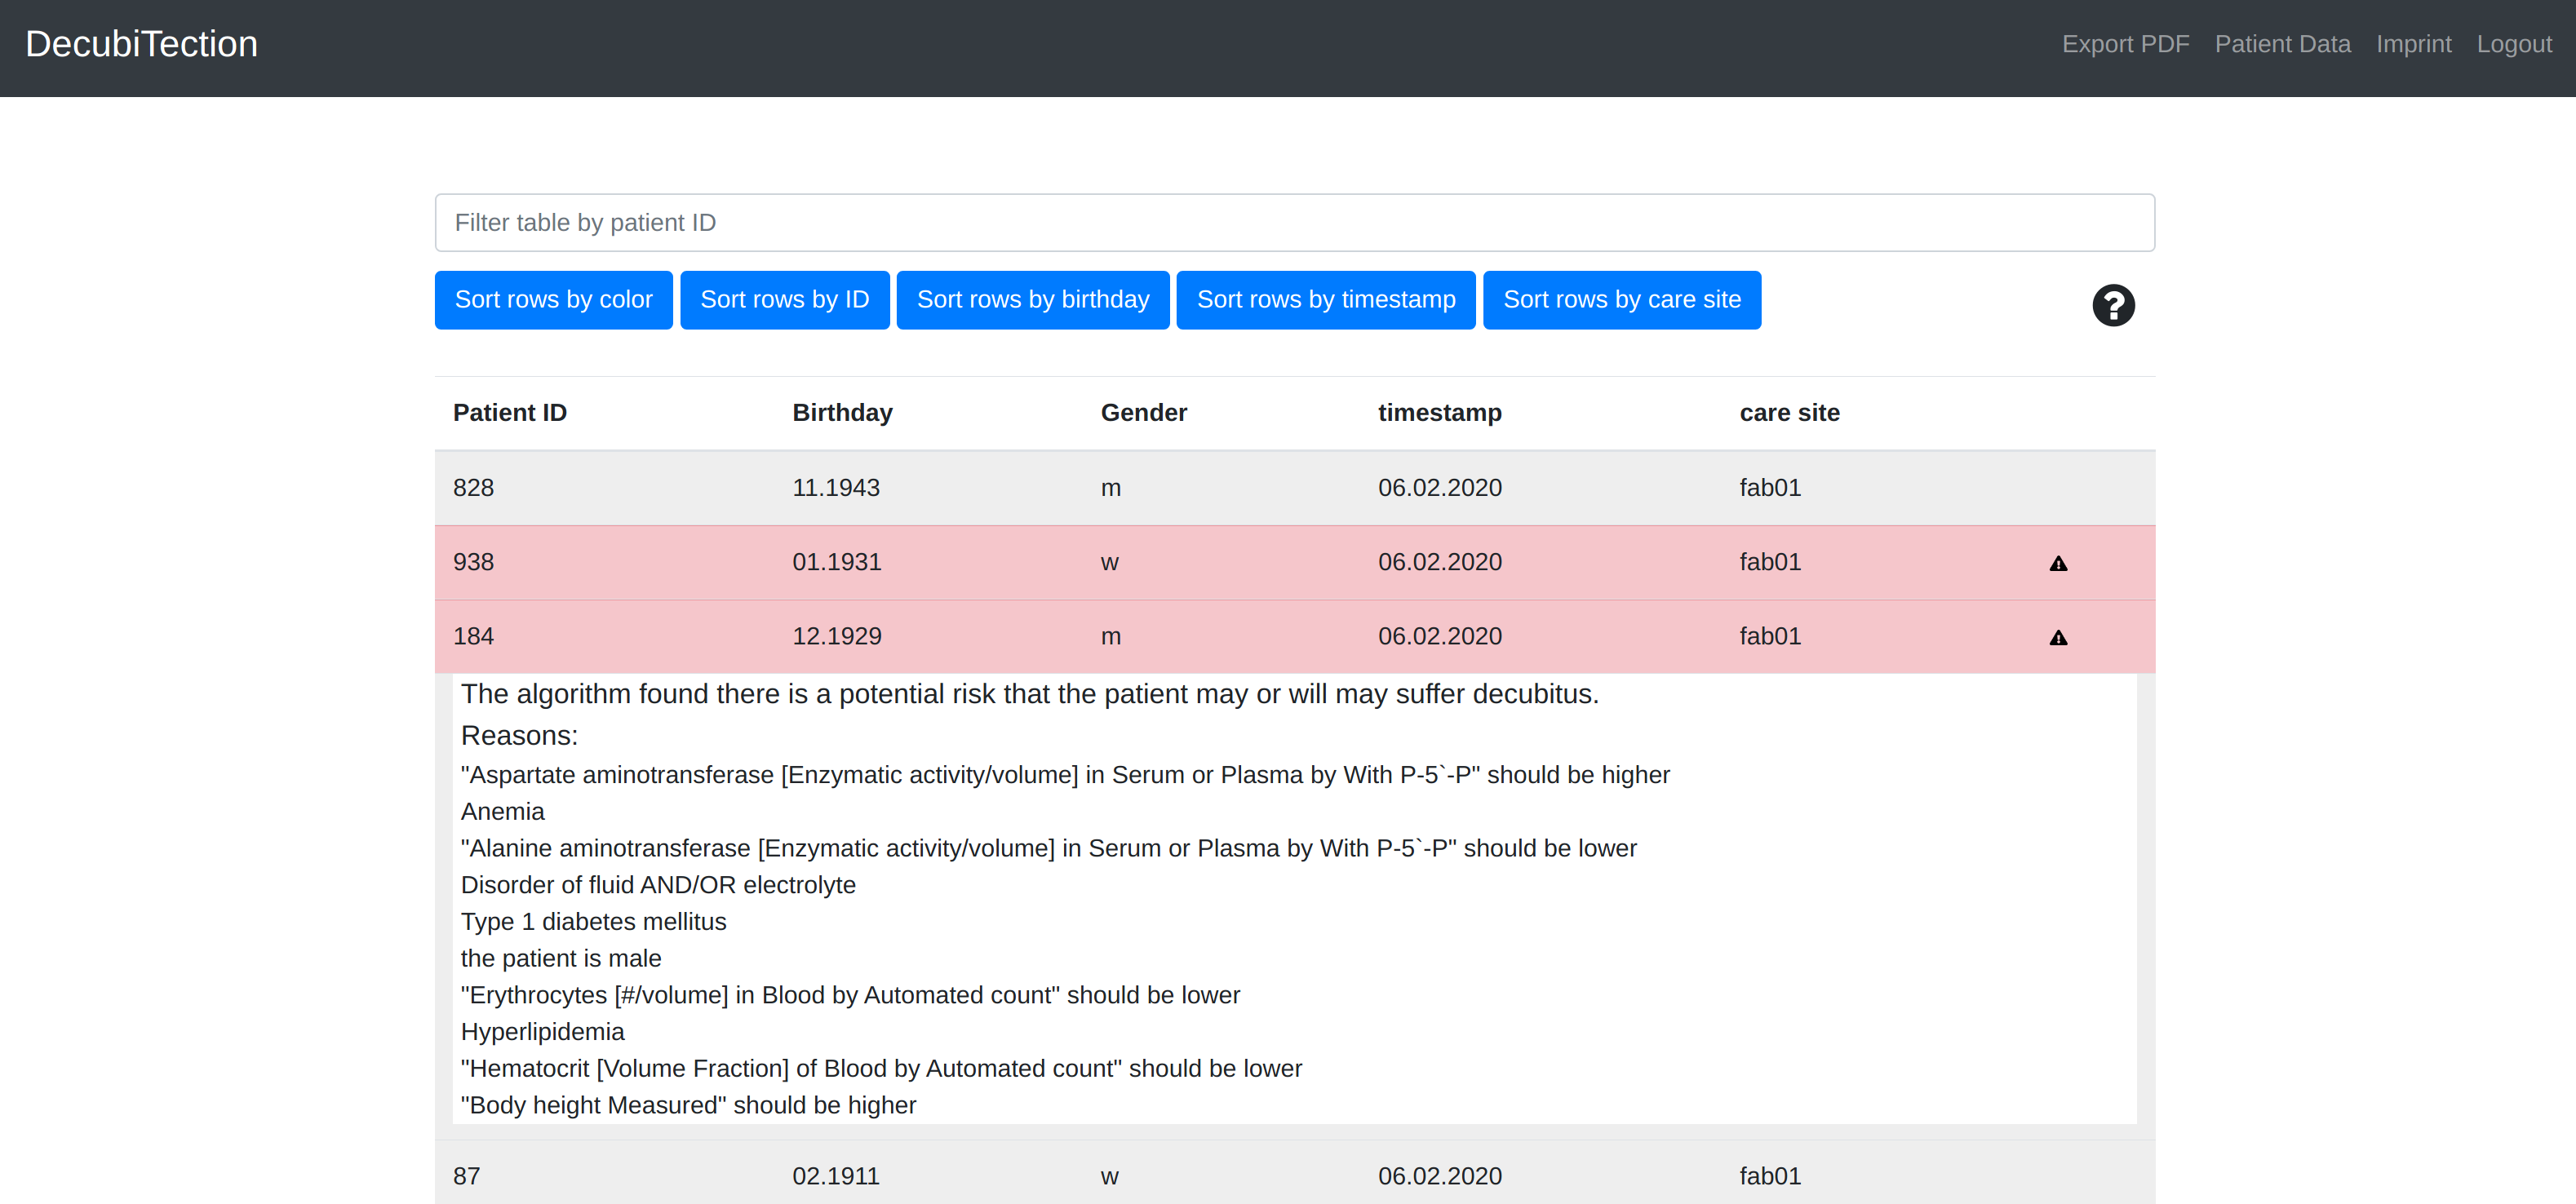
\includegraphics[width=15cm]{images/gray.png}}
    \caption{Most popular color theme of the front-end.}
    \label{fig:gray-color}
\end{figure}

\begin{figure}[htp]
    \centering
    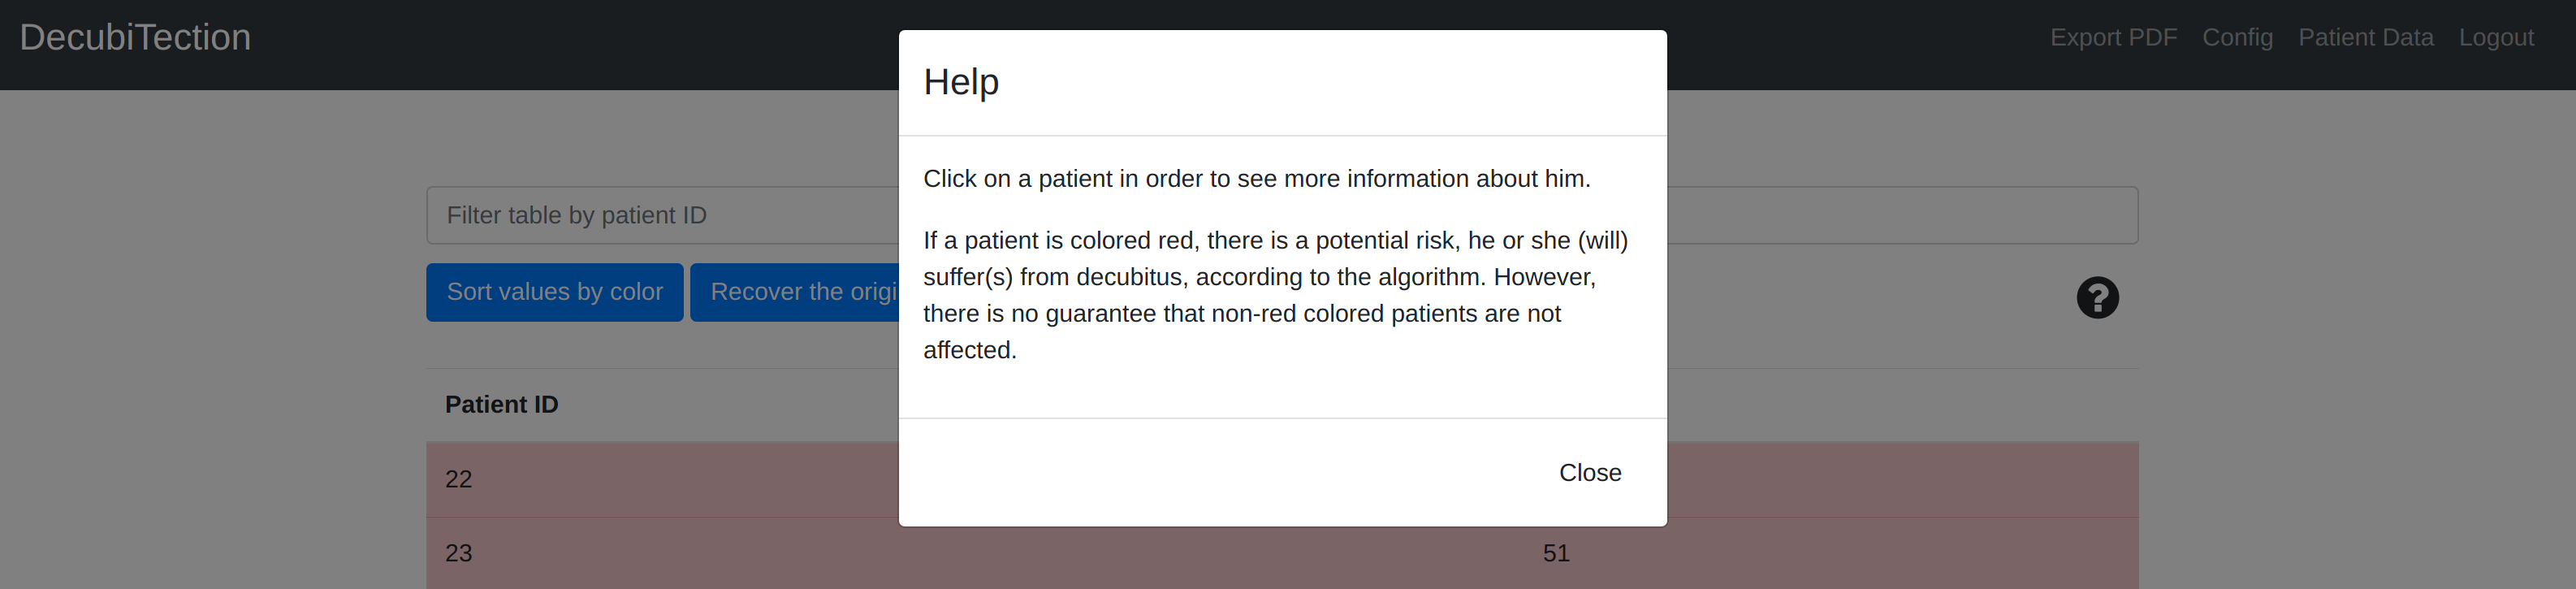
\includegraphics[width=15cm]{images/help.png}
    \caption{The help page of DecubiTection.}
    \label{fig:help}
\end{figure}

Though a web application brings many advantages, it contains a major disadvantage as well. 
Everyone inside the local network of the medical institution is able to access the front-end. 
We solved this by adding an authentication system, requiring valid credentials in order to access the front-end, depicted in \ref{fig:login}.
This decision matches the results of the questionnaire. 

\begin{figure}[htp]
    \centering
    \frame{
\includegraphics[width=15cm]{images/login.png}}
    \caption{The login page of DecubiTection.}
    \label{fig:login}
\end{figure}

\subsubsection{Content}
The results of the questionnaire showed that as general information, at least the patient ID and the birthday of the patient are required. 
Additionally, we added the patient's gender and the care-site, the patient is currently located in. 
In the front-end, one can filter patients by their ID and sort them by background colors. 
We included the option to save the results as PDF file as well. 
Hence a user is able to print the results. 

\subsubsection{Configuration}
There are different opinions, whether the front-end should include a configuration page e.g. for database credentials. 
We decided to not included such a page since it is not the front-end's users task to configure the software. 
In the current state, only an admin is able to configure the database settings and the credentials for authentication. 

\subsection{Back-End}
The cron job for the ETL-Process and the detection algorithm needs to be configured, according to several parameters. 
According to the results of the questionnaire, it is sufficient to include these parameters through command line parameters, e.g. \textit{python3 cron.py --db\_port=1234 --db\_host=localhost}.
Furthermore, the questionnaire showed the necessity for the following parameters:

\begin{itemize}
	\item cron interval
	\item for the database:
	\subitem username
	\subitem password
	\subitem host
	\subitem port
	\item location of the CSV files
\end{itemize}

Log files can be generated by redirecting the output of the software 
into a log-file. 